\documentclass[5p,times]{elsarticle} % Defence Technology (Elsevier); use mdpi.cls only if targeting MDPI Drones

\usepackage{graphicx}
\usepackage{tikz}
\usepackage[hidelinks,hypertexnames=false]{hyperref}
\usepackage{array}
\usepackage{float}
%\usepackage{lineno}
%\linenumbers

\usetikzlibrary{shapes.geometric, arrows.meta, positioning, fit}

\usepackage{amsmath,amssymb,amsfonts}
\usepackage{booktabs}
\usepackage{microtype}
\usepackage{url}
\urlstyle{tt}

\emergencystretch=3em

\begin{document}

\begin{frontmatter}

\title{A Hierarchical Virtual-Pursuit-Point Maneuver Interface for Close-Range Air Combat: Geometry Shaping via Learned Mode Routing among Frozen Specialists}

\author{}

\address{}

\begin{abstract}
Close-range air combat requires shaping advantageous engagement geometry under task- and opponent-dependent conditions. Classical virtual-pursuit-point (VPP) guidance remains interpretable because it commands an explicit geometric intermediate, but a single low-level VPP policy can still degenerate into target-chasing behavior once the engagement enters task-dependent post-merge regimes. We study a hierarchical maneuver interface that preserves the original three-dimensional VPP action head while adding a proximal-policy-optimization (PPO) high-level policy with two learned discrete routing actions for frozen head-on and crossing specialists. A deterministic geometry guard can additionally invoke a post-merge recovery profile that reuses the head-on specialist. Evaluation in a combat-only JSBSim scope with two tasks, two opponent configurations, and a crossing attack-zone limit of $60^\circ$ off the target's tail ($120^\circ$ target aspect angle) shows that the high-level policy is no longer weaker than the static oracle task gate on expert/head-on engagement ($0.6500$ vs.\ $0.5667$); the Wilson intervals overlap, so no statistical superiority is claimed. On end-to-end/head-on engagement, it remains slightly below the oracle ($0.9000$ vs.\ $0.9322$). Both methods obtain $0.7500$ on the canonical crossing-feasible check, but this is low-sample evidence ($N=4$ per split). A separate preregistered 24-scenario crossing envelope and three clean-import PPO training seeds meet a $-0.05$ practical preservation margin against a frozen fixed-VPP reference under both opponent splits. These results support a bounded claim: within a reproducible protocol, VPP advances from point chasing toward a combat-geometry shaping maneuver interface without changing the low-level action head.
\end{abstract}

\begin{keyword}
virtual-pursuit-point guidance; close-range air combat; hierarchical reinforcement learning; maneuver interface; combat geometry; task-label routing; PPO
\end{keyword}

\begin{highlights}
\item Hierarchical VPP preserves frozen 3-D action head and adds PPO mode routing.
\item PPO routing is no longer weaker than the static oracle on expert/head-on ($0.6500$ vs $0.5667$); overlapping Wilson intervals preclude a superiority claim.
\item End-to-end/head-on remains slightly below oracle ($0.9000$ vs $0.9322$); three paired oracle-only cases delimit the residual gap.
\item A disjoint 24-scenario crossing envelope and three clean-import PPO seeds meet a preregistered practical preservation screen against a frozen fixed-VPP reference.
\item Evaluation uses a reproducible JSBSim 6-DOF protocol with manifest-based provenance; exact configuration identifiers are recorded in the supplementary material.
\end{highlights}

\end{frontmatter}

\section{Introduction}

Virtual-pursuit-point (VPP) guidance is attractive in autonomous air combat because it expresses control intent through an explicit spatial intermediate rather than through opaque direct actuator commands. That explicitness, however, does not by itself guarantee tactically meaningful behavior. A single VPP policy can still degenerate into target chasing when it encounters task-dependent post-merge regimes in which the geometry needed for head-on recovery differs sharply from the geometry needed for crossing-feasible interception~\cite{xu2022ast}. Chen et al.~\cite{chen2019vpp} showed that virtual-target trajectory-following guidance with angle constraints can stabilize approach geometry, yet the challenge of regime-dependent behavior remains when a single policy must handle multiple engagement types~\cite{park2007,ratnoo2015}. The central question of this paper is therefore not whether VPP is usable as a control interface, but what evidence is required before it can be described as a genuine maneuver-decision interface that shapes favorable combat geometry.

Our answer is deliberately conservative. We do not introduce a new continuous action space or replace the original three-dimensional low-level VPP head. Instead, we preserve that low-level interface and move decision intelligence upward into a high-level policy with two learned discrete actions over frozen specialists. In the current evaluation wrapper, deterministic geometry guards can expose a third, post-merge recovery profile that reuses the head-on specialist rather than adding a third learned low-level policy. This design turns tactical mode selection into an auditable interface decision while retaining the geometric transparency of VPP at the low level~\cite{glanois2024}. This work directly extends the hierarchical architecture introduced in~\cite{lai2026aerospace}, but with two critical differences: (i) the low-level action head is strictly frozen rather than co-trained; (ii) the evaluation is conducted in JSBSim 6-DOF rather than in a simplified point-mass model, and the claim is explicitly bounded to a validated, reproducible protocol.

The contribution of this paper is not universal superiority over every baseline on every task. Rather, it is a reproducible and bounded positive result: the learned PPO high-level policy is no longer weaker than the oracle static gate on expert/head-on engagement, preserves the crossing specialist in the small crossing-feasible scope, and exposes a remaining end-to-end/head-on gap. A trained monolithic PPO baseline exists in the same environment but is outside the formal comparison; the claim is therefore one of sufficiency, not necessity. This makes the work suitable for presentation as a positive maneuver-interface study with an explicit bounded claim rather than as an open-ended tuning narrative.

The main contributions are fourfold:
\begin{itemize}
    \item a hierarchical VPP maneuver interface that preserves the original three-dimensional low-level action head while enabling task-dependent geometry production, with the frozen-head design preventing catastrophic forgetting of specialist geometry during high-level retraining;
    \item a constrained post-merge recovery guard that creates an explicit, auditable recovery profile by reusing the frozen head-on policy without retraining the low-level action space;
    \item a reproducible evaluation protocol built on validated evaluation execution, run manifest validation, and aggregate combat-geometry diagnostics;
    \item an experimentally bounded result: expert/head-on performance is no longer weaker than the oracle; canonical crossing evidence is an $N=4$ scope check but a separate disjoint crossing envelope supports practical preservation; and end-to-end/head-on remains slightly below oracle.
\end{itemize}

\section{Related Work}

\paragraph{Virtual pursuit points and geometry-aware guidance.}
Virtual-target and virtual-pursuit-point guidance methods provide a long-standing geometric framework for flight control because they separate high-level geometric intent from low-level stabilization~\cite{park2007,ratnoo2015}. Breivik and Fossen~\cite{breivik2005} formalized principles of guidance-based path following in two and three dimensions, and Sujit et al.~\cite{sujit2014} surveyed path-following algorithms for fixed-wing unmanned aerial vehicles. In aerial combat, tactical pursuit-point formulations further showed that behaviorally meaningful geometry can be expressed through intermediate spatial objectives rather than through direct end-to-end control~\cite{xu2022ast}. Our work follows this line but shifts the research question from hand-designed pursuit-point placement to learned routing among multiple geometry-producing VPP behaviors.

\paragraph{Learning-based maneuver decision.}
Reinforcement learning has been widely explored for UAV maneuver decision and autonomous close-range engagement~\cite{choi2023}. Soft actor-critic methods have been applied to aerial combat maneuvering~\cite{quan2026}, and variable-scale action strategies have been studied for close-range decision-making~\cite{wang2023aerospace}. DRL-based maneuver decisions for short-range air combat have been investigated by Yang et al.~\cite{yang2020access}, and Zhu et al.~\cite{zhu2024dt} demonstrated deep reinforcement learning for air combat games. Automatic opponent sampling has been used to improve dogfight decision-making~\cite{chen2025aerospace}, and deep Q-learning achieved human-level control in discrete domains~\cite{mnih2015}. Most such work focuses on algorithm choice, reward shaping, or modular policy design. By contrast, this study keeps the low-level VPP action interface fixed and asks whether hierarchical routing can turn that interface into a more behaviorally meaningful maneuver layer. In that sense, the novelty is not a new RL algorithm per se, but a new interface interpretation and evaluation discipline. Li et al.~\cite{li2022msddqn} proposed an MS-DDQN algorithm for short-range UCAV air combat, and Jiang et al.~\cite{jiang2025gail} explored generative adversarial imitation learning for autonomous maneuver decision-making. Fan et al.~\cite{fan2022a3c} employed an A3C-based method for UCAV air combat maneuver decisions, and Wang et al.~\cite{wang2024tactical} developed a deep learning approach for recognizing target tactical behavior intentions in air combat.

\paragraph{Hierarchical reinforcement learning and skill routing.}
Hierarchical RL decomposes complex decision problems into high-level policy selection over low-level sub-policies or options~\cite{sutton1999options}. The option-critic architecture provides a principled framework for learning options~\cite{bacon2017optioncritic}, and feudal networks enable hierarchical value decomposition~\cite{vezhnevets2017feudal}. In aerospace applications, HRL has been explored for multi-mode guidance and maneuver scheduling.
Guo et al.~\cite{guo2026hierarchical} proposed a hierarchical hybrid action reinforcement learning framework for beyond-visual-range air combat. Hou et al.~\cite{hou2023subtask} introduced subtask-masked curriculum learning for UAV maneuver decisions, and Zheng et al.~\cite{zheng2026wvr} applied curriculum learning to within-visual-range air combat in obstructed environments. The present work differs from standard HRL in that the low-level specialists are \emph{frozen} and \emph{interpretable} (they produce explicit 3D VPP geometry commands), and the high-level policy's action space is a discrete mode choice rather than a learned option termination. This makes the routing decision fully auditable, which aligns with assurance requirements for autonomous combat systems.

\paragraph{Interpretability and trustworthy autonomy.}
Recent interpretable-RL and assurance literature emphasizes that trustworthy autonomy depends not only on performance but also on whether the decision process can be inspected, audited, and stress-tested under reproducible conditions~\cite{glanois2024}. Safety assurance of machine learning for autonomous systems has been emphasized by Paterson et al.~\cite{paterson2025}, and explainable artificial intelligence has been surveyed by Gunning et al.~\cite{gunning2019}. Interpretable policies for autonomous driving have been learned by Paleja et al.~\cite{paleja2022}, and Han and Cheng~\cite{han2024smc} demonstrated interpretable DRL-based maneuver decisions for UCAV dogfight.. Our work addresses interpretability at the maneuver-interface layer: raw trajectories, mode-switch diagnostics, and aggregate combat-geometry diagnostics are used to determine whether the learned system is shaping geometry intentionally or merely exploiting incidental encounter dynamics.

\begin{table*}[htbp]
\centering
\small
\caption{Comparison of the proposed hierarchical VPP maneuver interface with representative guidance, DRL maneuver-decision, and HRL methods.}
\label{tab:comparison}
\resizebox{\textwidth}{!}{%
\begin{tabular}{@{}lp{2.6cm}cccp{2.4cm}p{2.4cm}@{}}
\toprule
\textbf{Method} & \textbf{Low-level control} & \textbf{Hierarchical} & \textbf{Frozen low-level} & \textbf{High-level routing} & \textbf{Simulator} & \textbf{Geometry interpretability} \\
\midrule
Park et al.~\cite{park2007} & Guidance law (path following) & No & N/A & None & Simplified model & High (analytical) \\
Ratnoo et al.~\cite{ratnoo2015} & Guidance law (trajectory shaping) & No & N/A & None & Simplified model & High (analytical) \\
Xu et al.~\cite{xu2022ast} & Tactical pursuit point (VPP) & No & N/A & None & Simplified model & High (spatial intermediate) \\
Yang et al.~\cite{yang2020access} & Direct actuator commands (DRL) & No & N/A & None & Simplified model & Low (end-to-end) \\
Zhu et al.~\cite{zhu2024dt} & Direct actuator commands (DRL) & No & N/A & None & Game engine & Low (end-to-end) \\
Wang et al.~\cite{wang2023aerospace} & Direct actuator commands (DRL) & No & N/A & None & Simplified model & Low (end-to-end) \\
Chen et al.~\cite{chen2023ppo} & PPO guidance law & No & N/A & None & Simplified model & Medium (policy-based) \\
Zheng et al.~\cite{zheng2023short} & Discrete action library (DRL) & No & N/A & None & Simplified model & Medium (action library) \\
Han et al.~\cite{han2024smc} & Direct actuator commands (DRL) & No & N/A & None & Simplified model & Medium (attention-based) \\
Guo et al.~\cite{guo2026hierarchical} & Hybrid action (DRL + discrete) & Yes & No & Co-trained & Simplified model & Medium (hybrid) \\
Lai et al.~\cite{lai2026aerospace} & VPP action head (3-D) & Yes & No & Co-trained & Simplified model & High (VPP intermediate) \\
\midrule
\textbf{This work} & \textbf{VPP action head (3-D)} & \textbf{Yes} & \textbf{Yes} & \textbf{Learned discrete mode} & \textbf{JSBSim 6-DOF} & \textbf{High (frozen VPP + auditability)} \\
\bottomrule
\end{tabular}
}
\end{table*}

\section{Materials and Methods}

\subsection{Hierarchical VPP Maneuver Interface}
\label{subsec:hierarchical_interface}

At the low level, all specialists retain the original three-dimensional VPP action head,
\begin{equation}
\mathbf{u}_t = [u_x, u_y, u_z]^\top \in [-1,1]^3,
\end{equation}
which produces a commanded virtual-pursuit-point position in the ego body frame,
\begin{equation}
\mathbf{p}_{\text{vpp}} = \mathbf{p}_{\text{ref}} + R_{\text{body}}^{\text{LOS}} \, [u_x \, d_{\text{ref}},\; u_y \, d_{\text{ref}},\; u_z \, \Delta h_{\text{max}}]^\top,
\end{equation}
where $\mathbf{p}_{\text{ref}}$ is a reference point on the line-of-sight (LOS) at distance $d_{\text{ref}} = 1000$\,m, $R_{\text{body}}^{\text{LOS}}$ is the rotation matrix from the LOS frame to the body frame, and $\Delta h_{\text{max}} = 300$\,m scales the altitude command. The VPP command is converted to aircraft control inputs via a guidance-to-actuator pipeline: the lateral component $u_y$ drives a commanded bank angle $\phi_{\text{cmd}}$ through a proportional-derivative (PD) controller with saturation, the vertical component $u_z$ drives a commanded load factor $n_{z,\text{cmd}}$ via a pitch-rate guidance law, and the axial component $u_x$ modulates thrust via a throttle PID. The complete signal flow from $\mathbf{u}_t$ to elevator/aileron/rudder/throttle is illustrated in Figure~\ref{fig:architecture}.

The main architectural change is therefore not the action dimensionality but the introduction of a high-level policy that selects which frozen low-level behavior should control the interface at each decision interval. This routing assignment reflects an architectural design choice motivated by the observed behavioral specialization of frozen specialists, rather than by a formal semantic mapping objective.

The learned high-level policy is PPO-based~\cite{chen2023ppo}. Its checkpoint has two learned discrete routing actions:
\begin{enumerate}
    \item Head-on specialist: the main frontal-engagement low-level policy;
    \item Crossing specialist: the low-level policy used for crossing-feasible interception;
\end{enumerate}
The evaluation wrapper can additionally expose a \emph{post-merge recovery profile} when deterministic degraded-geometry guards are active. This third evaluation mode is not a third learned action or a third low-level checkpoint: it reuses the head-on specialist under the configured recovery profile.
The oracle baseline, static oracle gate, is not a trainable high-level policy. It is a static task-label gate that routes by known scenario type. It serves as a direct comparison baseline for the question, ``Can the learned high-level policy preserve specialist behavior while making the correct routing decisions?'', but it is not presented as a universal upper bound.

Figure~\ref{fig:architecture} illustrates the hierarchical architecture. The PPO high-level policy chooses between two frozen low-level checkpoints, while the deterministic recovery guard can invoke a third evaluation profile over the head-on checkpoint. Both checkpoints share the same 3D VPP action head and interface with the JSBSim 6-DOF simulator.

\begin{figure*}[htbp]
\centering
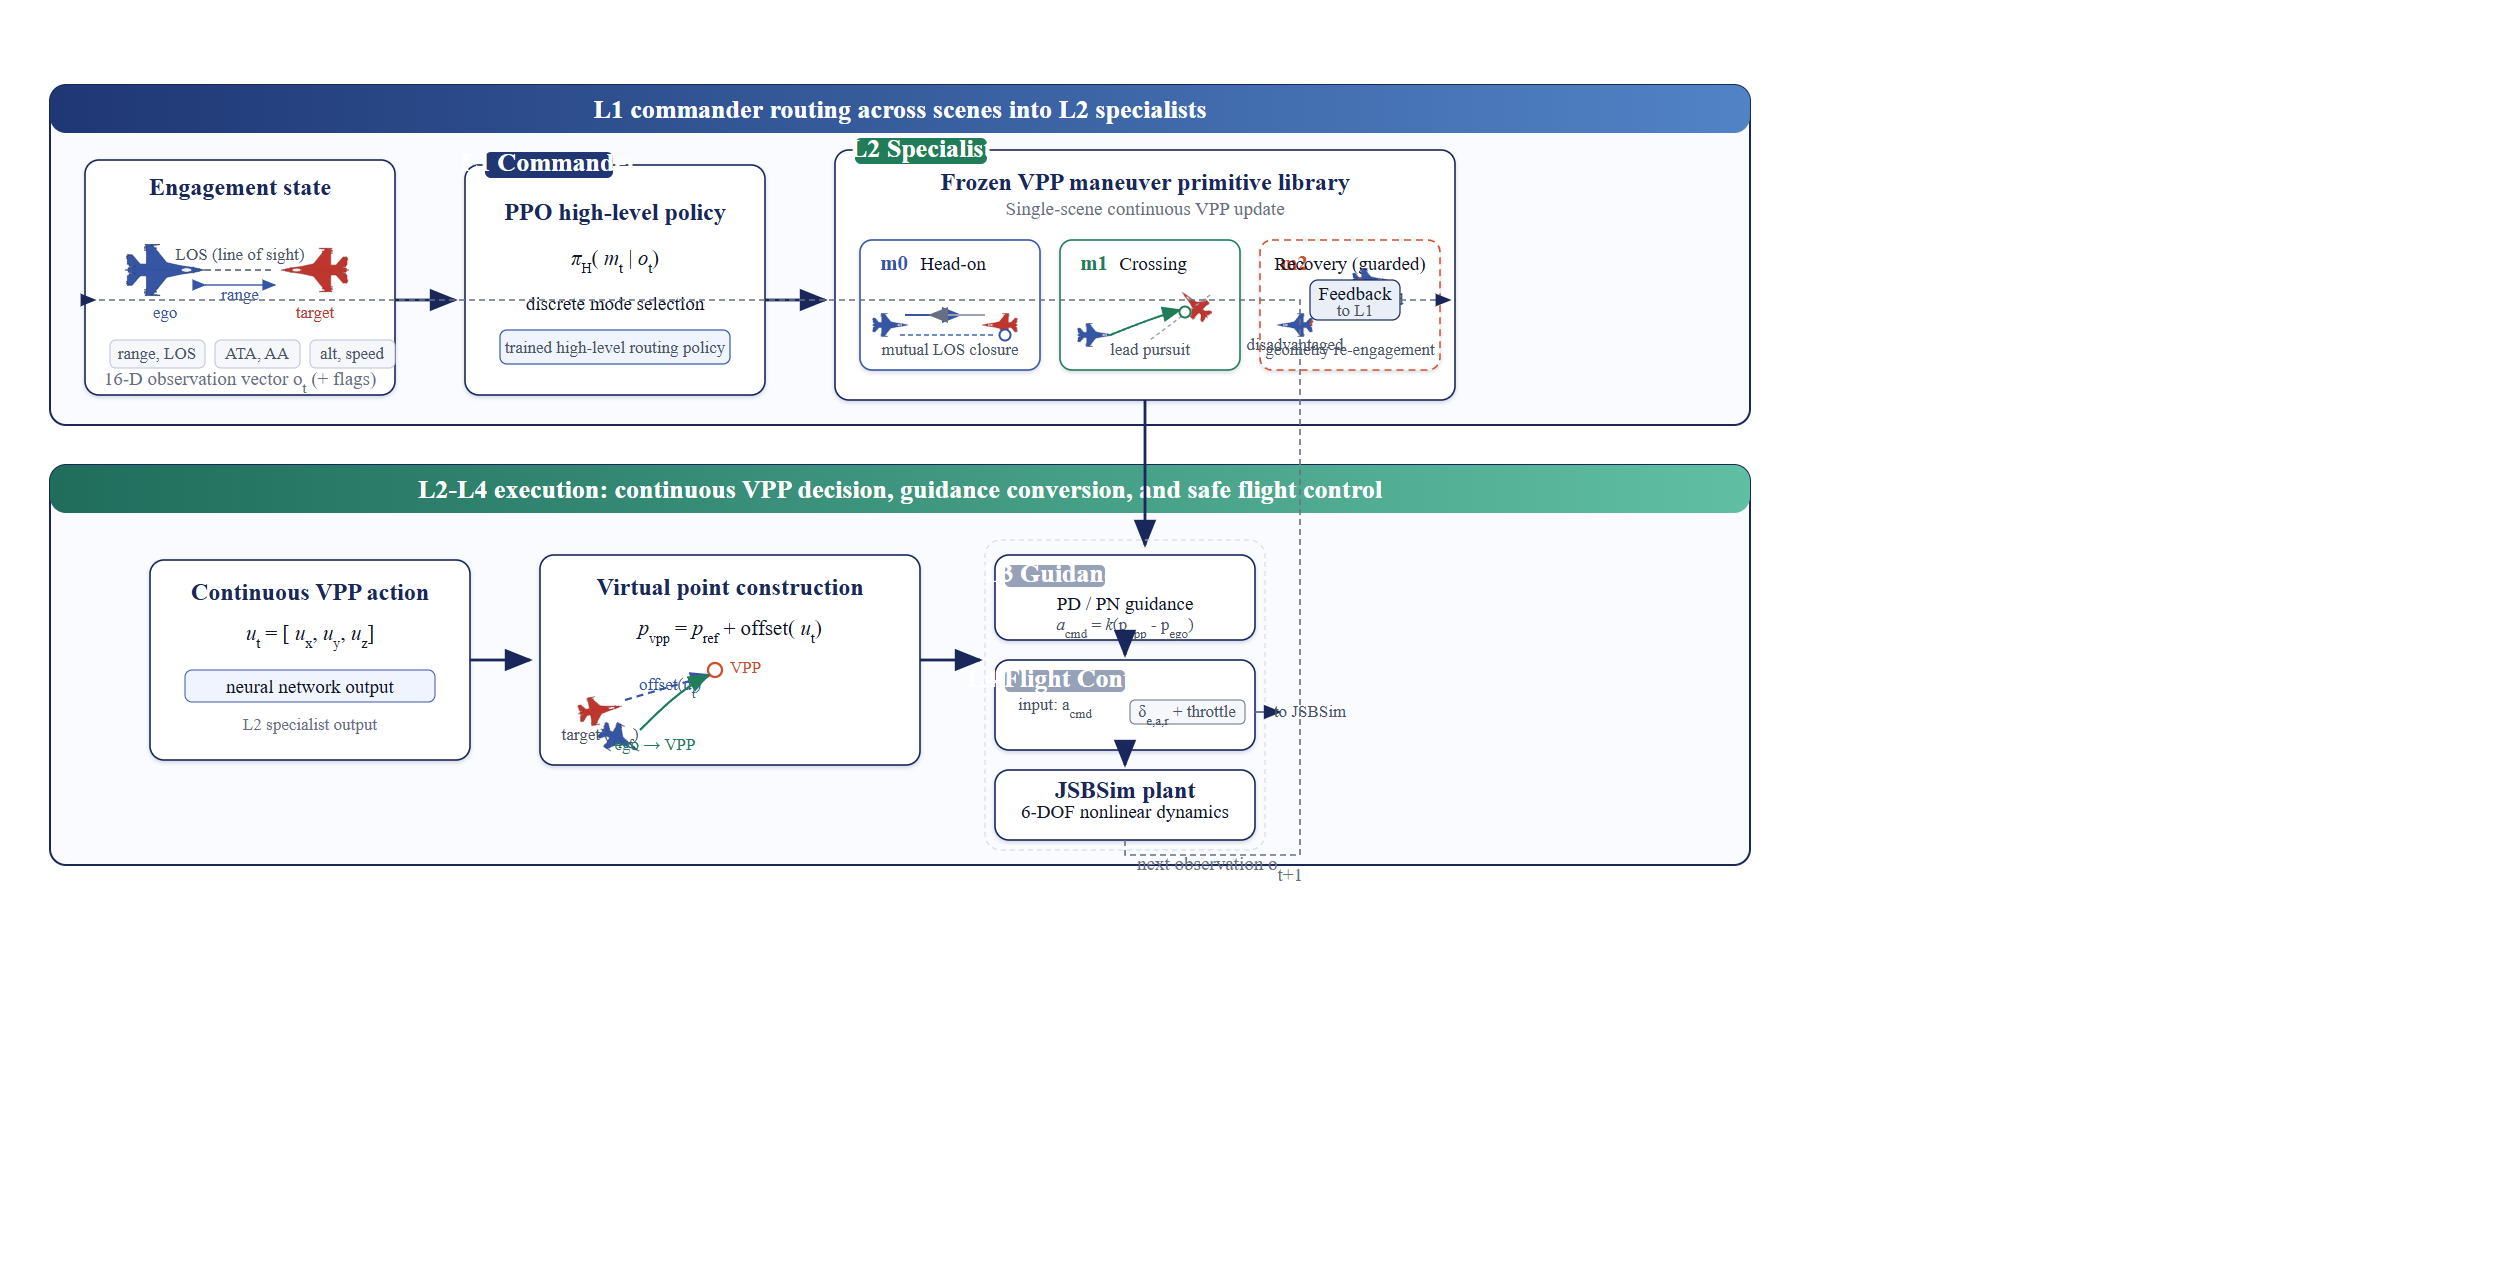
\includegraphics[width=0.9\textwidth]{figures/figure1_hierarchical_vpp_reference_submission_safe.png}
\caption{Hierarchical VPP maneuver interface. The PPO high-level policy routes among two frozen low-level specialists (head-on and crossing) and a post-merge recovery profile that conditionally reuses the head-on specialist under explicit geometry guards. All share the same three-dimensional VPP action head and are evaluated in the JSBSim 6-DOF simulator.}
\label{fig:architecture}
\end{figure*}

\subsubsection{Opponent Models and Evaluation Splits}

Two opponent policies are used to test generalization across different behavioral regimes.

expert opponent: a scripted energy-management opponent that performs defensive basic fighter maneuvers (BFM) including high-\textit{yo-yo} extensions and spiral descent turns to preserve specific energy while denying a firing solution. It is not a learning-based agent; its maneuver sequence is drawn from a hand-crafted state machine that reacts to relative geometry (range, aspect angle, and closure rate) with deterministic energy-priority logic. Its task-level outcomes are reported in Table~\ref{tab:main_results}.

end-to-end opponent: a monolithic PPO policy trained without hierarchical routing, using the same observation space and JSBSim F-16-like aircraft model. It represents a fully learned opponent that does not use frozen specialists or task-label routing. The distinct outcome pattern on this split is reported separately in Table~\ref{tab:main_results}; the paper does not attribute that pattern to a single causal property of the opponent.

Deep reinforcement learning for path planning in dynamic environments has been demonstrated by Yan et al.~\cite{yan2020path}. Both opponents use the same JSBSim aircraft model (F-16-like configuration with mass $m = 9295$\,kg, reference wing area $S = 27.87$\,m$^2$, sea-level thrust $T_{\text{SL}} = 76.3$\,kN, and maximum load factor $n_{z,\max} = 9.0$). Full aerodynamic tables and engine model parameters are archived in the supplementary configuration snapshots. Multi-agent reinforcement learning with target position prediction has been applied to within-visual-range air combat by Kong et al.~\cite{kong2020mappo}, and Liu et al.~\cite{liu2022mappo} studied MAPPO algorithms for beyond-visual-range cooperative air combat.

\subsubsection{Low-Level Specialist Training}

The two frozen specialists use the same JSBSim 6-DOF aircraft model and low-level flight-control profile (bank-angle protection with altitude-hold lift smoothing), but their checkpoint observation contracts differ. The head-on checkpoint accepts a 19-dimensional input, whereas the historical crossing-v3 checkpoint accepts an 18-dimensional input; both emit the same three-dimensional VPP action. During canonical evaluation, the environment emits the 19-dimensional runtime observation and a compatibility adapter applies the crossing checkpoint's historical 18-dimensional contract. The baseline network is a two-layer MLP with 128 hidden units per layer and \texttt{tanh} activation, trained with PPO ($\gamma=0.99$, $\lambda=0.95$, clip $0.2$, learning rate $3\times 10^{-4}$, 2\,048 rollout steps, minibatch size 256, 10 update epochs, entropy coefficient $0.01$). Full hyperparameters are archived in the supplementary configuration snapshot.

The selected \emph{head-on specialist} checkpoint records a cold start (\texttt{warm\_start.enabled=false}). Its configuration budget was 32\,768 environment steps, while the selected \texttt{best.pt} checkpoint was written at 8\,192 steps. Its combat-finetune task weights were $w_{\text{head-on}}=2.0$ and $w_{\text{crossing}}=1.0$. We report the selected-checkpoint metadata rather than treating the configured budget as completed training.

The \emph{crossing specialist} checkpoint also records a cold start (\texttt{warm\_start.enabled=false}) and 65\,536 training steps, with task weights $w_{\text{head-on}}=1.0$ and $w_{\text{crossing}}=2.0$. Checkpoint selection uses a task-gated metric: the crossing-feasible expert win rate must pass four geometry gates ($\text{win\_rate}\ge 0.5$, $\text{hp\_advantage}\ge 0$, $\text{timeout\_rate}\ge 0.2$, $\text{out\_of\_bounds\_rate}\le 0.7$) before the win rate is used as the selection objective.

The \emph{post-merge recovery profile} is not a separately trained policy. It is a deterministic runtime profile that reuses the head-on checkpoint when configured degraded-geometry guards are active. This design keeps the action space frozen while adding a constrained recovery path without claiming a third specialist or a third learned PPO action.

\subsubsection{High-Level Policy Observation Space}

The PPO high-level policy receives a 16-dimensional base observation vector at each high-level decision epoch:
\begin{equation}
\begin{split}
\mathbf{o}_t = [&r, \dot{r}, \Delta h, \Delta v, \sin\psi_{\text{LOS}}, \cos\psi_{\text{LOS}}, \sin\theta_{\text{LOS}}, \cos\theta_{\text{LOS}}, \\
&\sin\text{ATA}, \cos\text{ATA}, \sin\text{AA}, \cos\text{AA}, v_{\text{ego}}, v_{\text{tgt}}, h_{\text{ego}}, h_{\text{tgt}}]^\top,
\end{split}
\end{equation}
where $r$ is relative range, $\dot{r}$ is range rate, $\Delta h$ and $\Delta v$ are altitude and speed differentials, $\psi_{\text{LOS}}$ and $\theta_{\text{LOS}}$ are line-of-sight azimuth and elevation (geometric definitions: $\psi_{\text{LOS}} = \arctan2(\Delta y, \Delta x)$, $\theta_{\text{LOS}} = \arctan2(\Delta z, \sqrt{\Delta x^2 + \Delta y^2})$), ATA is aspect angle, and AA is antenna angle. The formal evaluations append three binary indicators: one crossing-task indicator and two opponent-stage indicators (expert and end-to-end), yielding a 19-dimensional policy input. These indicators are recorded in the resolved configuration and observation audit; their isolated causal contribution is not evaluated in this paper.

\subsection{Reward Structure}

The PPO high-level policy receives a task-aware reward designed to favor favorable engagement geometry rather than purely terminal win/loss outcomes. At each step, the reward is
\begin{equation}
\begin{aligned}
r_t =&\; r_{\text{win}} \cdot \mathbb{1}_{\text{win}} + r_{\text{loss}} \cdot \mathbb{1}_{\text{loss}} + r_{\text{terminal}} \\
    &+ r_{\text{range}} + r_{\text{angle}} + r_{\text{smooth}} + r_{\text{sat}} \\
    &+ r_{\text{turn}} + r_{\text{closing}} + r_{\text{alive}} + r_{\text{overshoot}} \\
    &+ r_{\text{boundary}} + r_{\text{attack}} + r_{\text{attack\_score}},
\end{aligned}
\end{equation}
where the terminal and geometric terms are defined as follows. Terminal win/loss terms are $r_{\text{win}} = +1.0$ and $r_{\text{loss}} = -1.0$; an additional terminal bonus $r_{\text{terminal}} = +400$ for success and $-300$ for failure is added when the episode terminates. The range term $r_{\text{range}}$ rewards keeping the opponent inside an ideal engagement band $[r_{\min}, r_{\max}]$ (specialist-specific: $[700, 1100]$~m for the base policy, $[800, 1200]$~m for the head-on specialist, $[700, 1100]$~m for the crossing specialist):
\begin{equation}
r_{\text{range}} =
\begin{cases}
+0.3 & \text{if } r_{\min} \le r \le r_{\max}, \\
-0.6 \cdot \frac{r_{\min} - r}{r_{\min}} & \text{if } r < r_{\min}, \\
-0.6 \cdot \min\!\left(1, \frac{r - r_{\max}}{4000 - r_{\max}}\right) & \text{if } r > r_{\max},
\end{cases}
\end{equation}
with weight $w_{\text{range}} = 0.6$. The angle term $r_{\text{angle}}$ with weight $w_{\text{angle}} = 0.9$ biases the line-of-sight angle $\theta_{\text{LOS}}$ toward the forward quadrant:
\begin{equation}
r_{\text{angle}} =
\begin{cases}
+0.9 \cdot \frac{\theta_{\text{LOS}}}{45^{\circ}} & \text{if } \theta_{\text{LOS}} < 45^{\circ}, \\
+0.9 \cdot \left(1 - \frac{\theta_{\text{LOS}} - 45^{\circ}}{90^{\circ}}\right) & \text{if } 45^{\circ} \le \theta_{\text{LOS}} \le 135^{\circ}, \\
-0.9 & \text{if } \theta_{\text{LOS}} > 135^{\circ}.
\end{cases}
\end{equation}
Smoothness $r_{\text{smooth}} = -0.2 \cdot \lVert \mathbf{u}_t - \mathbf{u}_{t-1} \rVert^2$ penalizes action jitter; saturation $r_{\text{sat}} = -0.5 \cdot \mathbb{1}_{\text{sat}}$ penalizes control saturation (load-factor, roll-rate, or throttle limits); turn-rate $r_{\text{turn}} = -0.5 \cdot \max(0, \lvert \dot{\phi} \rvert - 150^{\circ}/\text{s})$ discourages excessive bank-angle rate; closing $r_{\text{closing}} = -0.1 \cdot \max(0, -\dot{r})$ penalizes increasing range; alive $r_{\text{alive}} = +0.02$ per step is a survival bonus; overshoot $r_{\text{overshoot}} = -1.0 \cdot \mathbb{1}_{\text{over}}$ fires when the aircraft passes the target without a kill; boundary $r_{\text{boundary}} = -0.3 \cdot \mathbb{1}_{\text{oob}}$ fires on out-of-bounds or altitude violation. The attack-zone terms $r_{\text{attack}} = +0.3$ (inside zone, $\text{off-the-tail} \le 60^{\circ}$) and $r_{\text{attack\_score}} = +0.5$ (score contribution) are active only during combat-finetune training of the head-on specialist. This reward structure was frozen before the constrained repair began and was not modified during recovery-profile retraining. All weight values are fixed across the training pipeline and are not tuned per specialist.

\subsection{Formal Repair and Residual Boundary}

The learned high-level policy, denoted $\pi_{\theta}^{*}$, is the result of a constrained repair sequence that targeted degraded-geometry head-on failure without reopening the action space or retraining the low-level specialist set.

\textbf{Methodological limitation: iterative repair exposure.} The recovery profile thresholds were determined from failure-mode analysis on the same evaluation scenarios that were later used for formal reporting. This constitutes iterative debugging on the evaluation set, which may inflate the reported repair performance. No independent validation split was used during threshold selection. The thresholds were frozen before the final validated evaluation run, but the iterative exposure means the reported numbers should be interpreted as a sufficiency demonstration rather than as an unbiased generalization estimate. A fresh held-out scenario set was reserved for future robustness validation.

\textbf{Repair target.} In preliminary evaluation, the unmodified PPO high-level policy exhibited systematic ego-crash or out-of-bounds on head-on engagement against the expert opponent scenarios with large initial lateral offset and negative altitude differential. The failure mode was traced to premature commitment to the head-on specialist before the engagement geometry had stabilized.

\textbf{Repair mechanism.} The constrained repair added a deterministic post-merge recovery profile (Section~\ref{subsec:hierarchical_interface}) to the evaluation wrapper. The profile reuses the head-on checkpoint when its configured degraded-geometry guards are active; it is not an independently trained specialist or a third learned PPO action. The guard configuration was frozen before the canonical evaluation; no sensitivity or threshold-optimality claim is made in this paper.

The policy is now frozen. Further work on the remaining residuals is intentionally excluded from the current publication-facing evaluation set and is reserved for a separate future low-level recovery study.

\subsection{Formal Evaluation Scope}

All headline numbers in this paper come from completed clean-worktree evaluation runs with a resolved configuration, run manifest, raw episode records, and a valid artifact contract. The scope is fixed as follows:
\begin{itemize}
    \item tasks: head-on and crossing-feasible;
    \item opponent splits: expert opponent and end-to-end opponent;
    \item backend: JSBSim;
    \item crossing attack-zone limit: maximum off-the-tail angle $60^\circ$ (i.e., $120^\circ$ target aspect angle);
    \item scenario family: evaluation set head-on set plus the fixed crossing scope.
\end{itemize}

The canonical dual-opponent evidence comprises two clean JSBSim runs executed from the same frozen code revision:
\begin{itemize}
    \item expert formal run (Expert-20260705);
    \item end-to-end formal run (EndToEnd-20260705).
\end{itemize}
Both runs were generated at clean commit \texttt{9a9f9bf6d685}. Their full directory identifiers and artifact hashes are retained in the reproduction bundle and in the accompanying authoritative artifact index. Each includes run metadata, resolved configuration files, raw episode data, aggregate statistics, and artifact validation. A further preregistered crossing-only RQ1 envelope is reported separately in Supplementary Table~S3 and Figure~S3; it freezes the comparison methods and evaluates 24 disjoint crossing scenarios under both opponents.

\subsection{Evaluation Metrics}

The primary metric is task-level win rate, defined as the number of wins divided by the number of resolved episodes (wins plus losses). Episodes that end in an unresolved draw, an unqualified timeout, or an unlabeled timeout are excluded from the win-rate denominator. They are counted in the reported episode total $N_{\text{total}}$ but not in the resolved count $N_{\text{resolved}}$. This distinction is material because one task (end-to-end / head-on / oracle) reports 60 total episodes but 59 resolved.

We also inspect combat-geometry diagnostics, mode fractions, simulator fallback count, and terminal-event summaries. The canonical headline crossing cells contain only four scenarios per split and remain scope-preservation checks. To test whether that limitation masks a fixed-reference routing deficit, the preregistered RQ1 supplement evaluates a disjoint 24-scenario crossing envelope and then three independent PPO training seeds. It reports paired differences, Wilson intervals, mode fractions, and terminal events in Supplementary Table~S3 and Figure~S3. Its $-0.05$ preservation threshold is a practical gate, not a superiority test.

\subsection{Evaluation Protocol Summary}
\label{subsec:protocol_summary}

Table~\ref{tab:protocol} summarizes the key experimental parameters.

\begin{table*}[htbp]
\centering
\small
\caption{Evaluation protocol summary.}
\label{tab:protocol}
\begin{tabular}{@{}lp{12cm}@{}}
\toprule
Parameter & Value \\
\midrule
High-level observation & 16 base features (relative geometry + kinematics) plus three task/opponent indicators (19 total) \\
Action head & $[u_x, u_y, u_z]^\top \in [-1,1]^3$ (3D VPP command) \\
Low-level policies & 2 frozen checkpoints: head-on (19-D input) and crossing-v3 (18-D input); recovery is a guard-mediated profile over head-on \\
High-level policy & PPO with a 19-D input, two learned actions, and 128/128 hidden layers; the guard-mediated profile is outside the learned action head \\
Decision cadence & JSBSim integration at 60 Hz; high-level routing action every 0.2 s (5 Hz), held for 12 integration steps \\
Episode cap & 512 high-level steps (102.4 s) \\
Simulator & JSBSim high-fidelity 6-DOF \\
Evaluation scope & 2 tasks $\times$ 2 opponent splits; 60 head-on scenarios per split, 4 crossing per split \\
Crossing attack-zone limit & $60^\circ$ off the target's tail (i.e., $120^\circ$ target aspect angle) \\
PPO learning rate & $3 \times 10^{-4}$ (Adam) \\
PPO discount factor $\gamma$ & $0.99$ \\
GAE-Lambda $\lambda$ & $0.95$ \\
Clip range $\epsilon$ & $0.2$ \\
Steps per update & $2048$ \\
Entropy coefficient & $0.01$ \\
Resolved-episode rule & Wins + losses; draws and unqualified timeouts excluded from denominator \\
\bottomrule
\end{tabular}
\end{table*}

\begin{figure}[htbp]
\centering
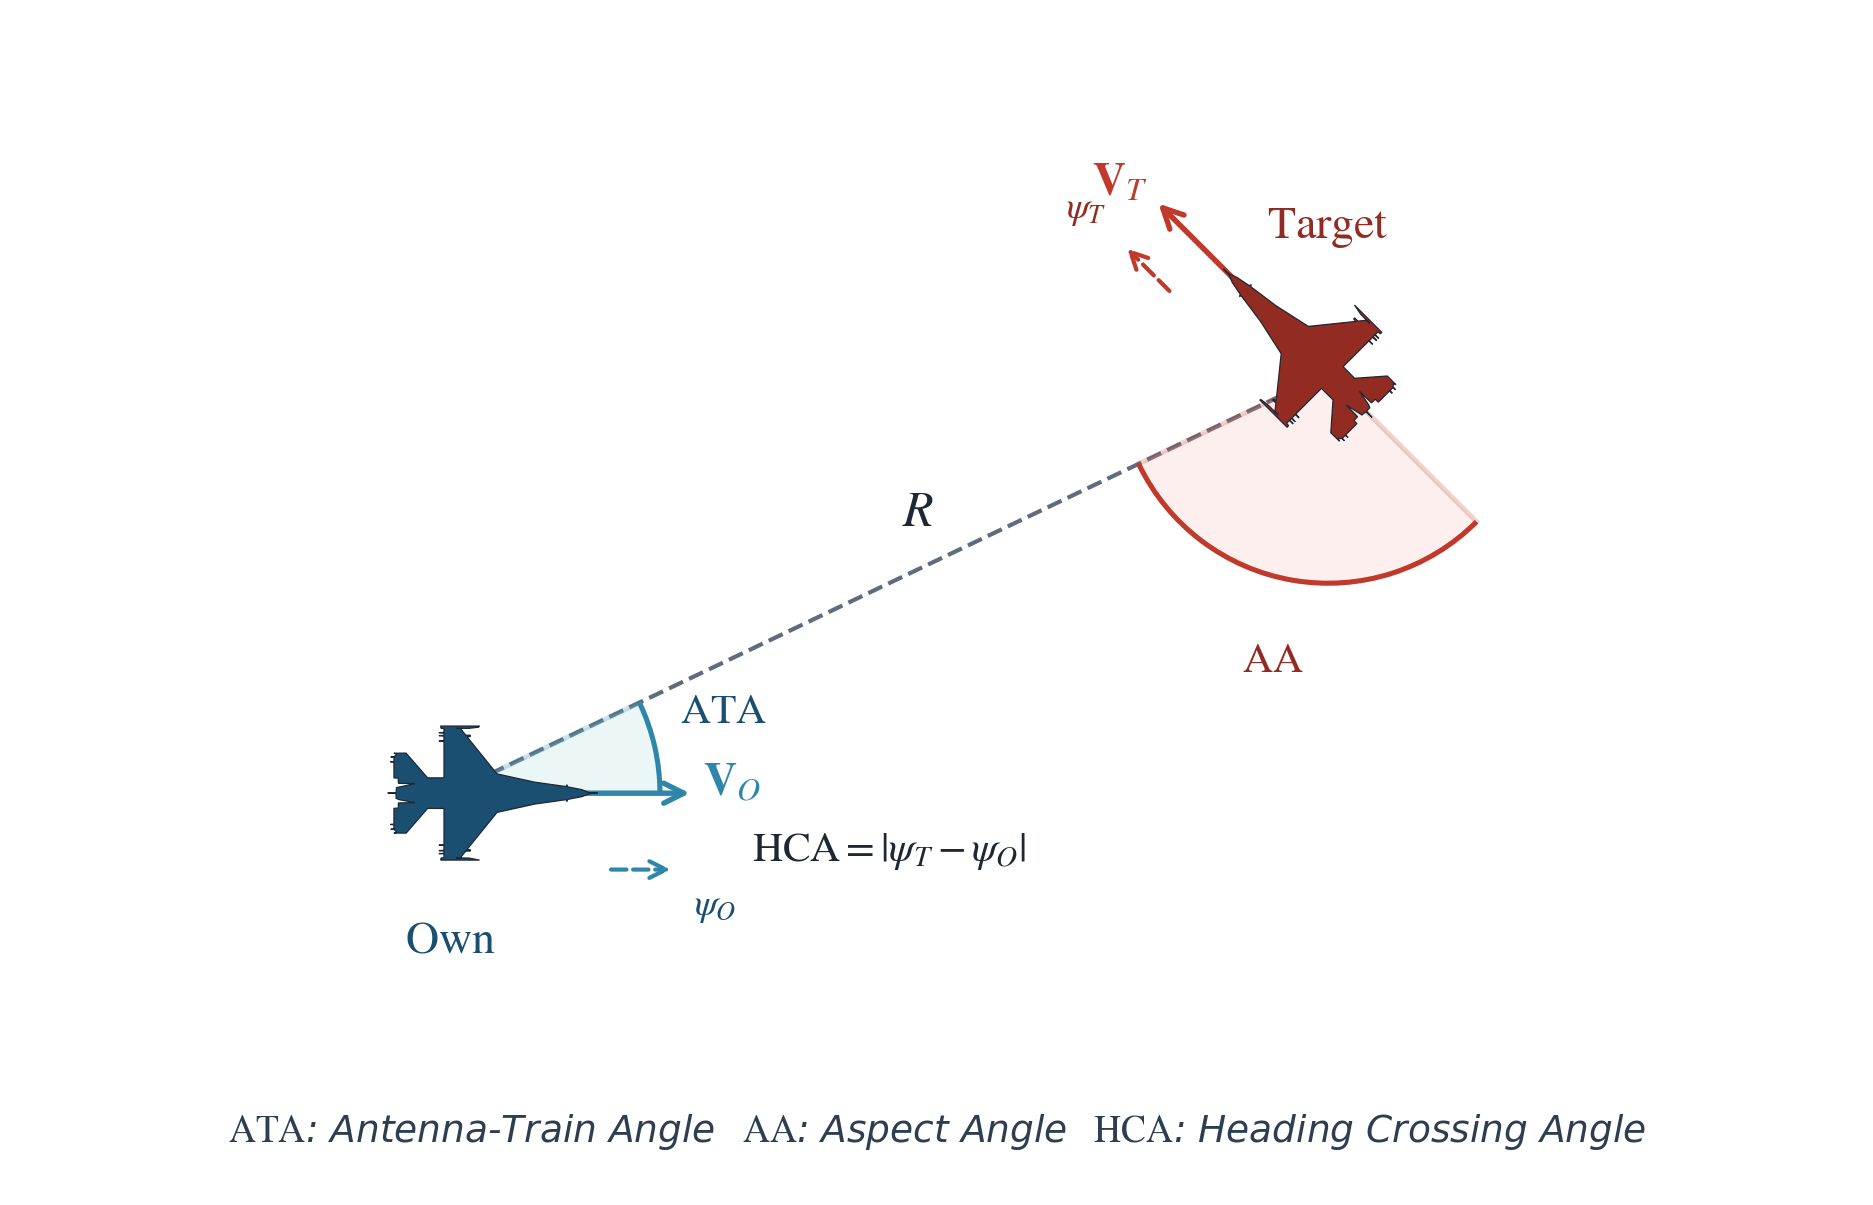
\includegraphics[width=0.85\columnwidth]{figures/figure1_air_combat_geometry.png}
\caption{Air combat engagement geometry. The observation vector $\mathbf{o}_t$ comprises relative range $r$, range rate $\dot{r}$, line-of-sight azimuth $\psi_{\mathrm{LOS}}$ and elevation $\theta_{\mathrm{LOS}}$, aspect angle ATA, antenna angle AA, and ego/target speed and altitude differentials.}
\label{fig:combat_geometry}
\end{figure}

\subsection{Implementation and Reproducibility Details}

JSBSim integrates the flight dynamics at 60 Hz. The high-level routing action is selected every 0.2 s (5 Hz) and held for 12 integration steps; an episode is capped at 512 high-level steps (102.4 s), or terminates earlier upon win, loss, or out-of-bounds. The frozen PPO checkpoint uses a 19-dimensional input, two learned actions, and a fully connected 128/128 hidden-layer architecture. The deterministic recovery profile is applied by the evaluation wrapper and does not add a learned PPO action. The dual-opponent headline comparison reports one frozen checkpoint; the separate RQ1 supplement evaluates three independently trained, clean-import PPO seeds without replacing that headline comparison. Both low-level checkpoint policies were frozen before high-level policy training and were not updated during PPO training. The JSBSim aircraft model is the F-16-like configuration provided with the open-source JSBSim reference data package; full model parameters are archived in the supplementary configuration snapshots.

\begin{figure*}[htbp]
\centering
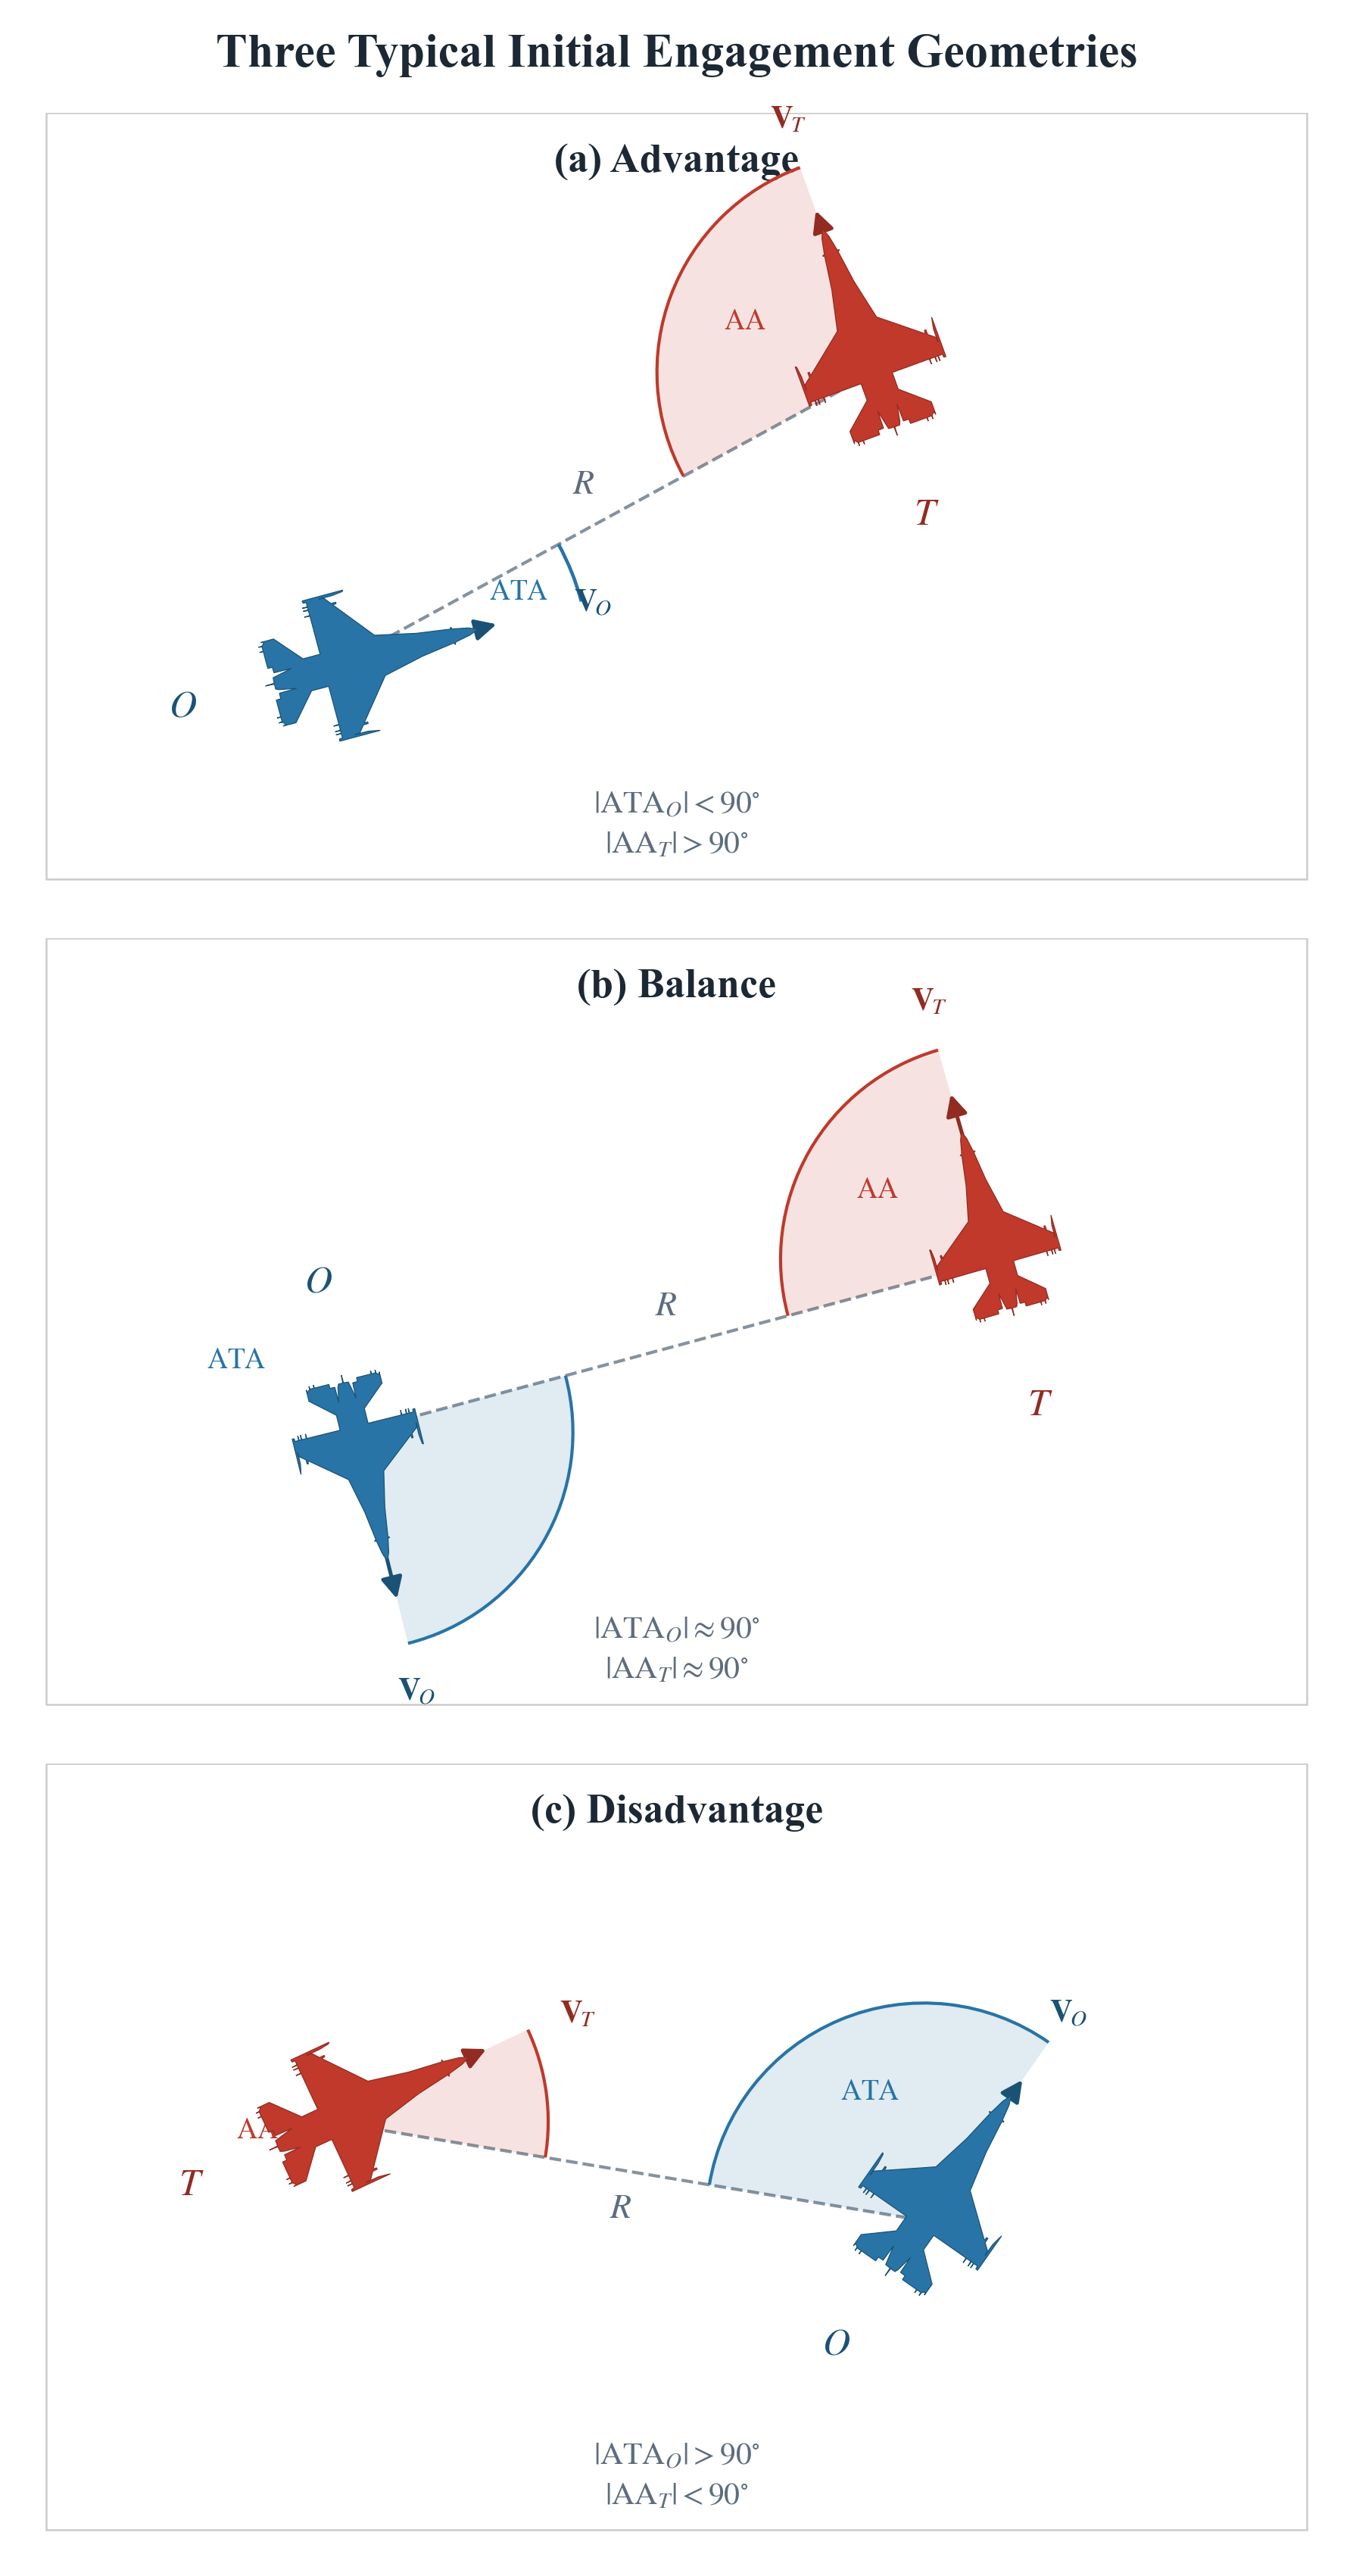
\includegraphics[width=\textwidth, height=0.8\textheight, keepaspectratio]{figures/figure2_three_initial_situations.png}
\caption{Three initial engagement situations used in the evaluation protocol: (left) head-on with equal speed and altitude; (middle) crossing with lateral offset; (right) head-on with altitude differential and negative lateral offset. The scenario family covers the decisive geometry regimes that distinguish specialist behavior.}
\label{fig:initial_situations}
\end{figure*}

\section{Results}

\subsection{Authoritative Formal Comparison}

In Table~\ref{tab:main_results}, \textbf{PPO} denotes the learned high-level policy with two discrete routing actions over frozen low-level checkpoints; the deterministic recovery profile is an evaluation-wrapper constraint rather than a third learned policy. \textbf{Oracle} denotes the static task-label gate that routes by known scenario type. Win rates are proportions over resolved episodes, as defined in Supplementary Note~A. The table reports the canonical frozen policy checkpoint and dual-opponent headline comparison. Training-seed variability is evaluated separately, without replacing these headline numbers, in Supplementary Table~S3 and Figure~S3.

On expert/head-on, PPO wins $39/60=0.6500$ resolved episodes versus $34/60=0.5667$ for Oracle. Their Wilson intervals overlap, so the result is reported only as ``no longer weaker than the oracle,'' not as a statistically significant improvement. On end-to-end/head-on, PPO wins $54/60=0.9000$ versus $55/59=0.9322$ for Oracle; the one unresolved Oracle draw is excluded from its denominator. The canonical crossing-feasible result is $3/4=0.7500$ for both methods and both opponent splits, so it remains a four-scenario scope check. Separately, the 24-scenario RQ1 crossing envelope meets a preregistered practical preservation screen against a fixed head-on VPP reference under both opponents; all six cells from three independent PPO seeds also meet that screen. These auxiliary results are preservation evidence within the stated envelope, not broad generalization or superiority evidence.

The numerical values in Table~\ref{tab:main_results} reproduce Supplementary Table~S1 and Supplementary Note~A. The exact run identifiers, resolved configurations, artifact contracts, and raw episode records are identified in Section~\ref{subsec:protocol_summary} and the Data Availability statement.

\begin{table*}[htbp]
\centering
\caption{Win-rate comparison between oracle static gate (Oracle) and learned PPO high-level policy (PPO). Win rates are reported as proportions over resolved episodes. Wilson score 95\% confidence intervals are reported for binomial proportions. Crossing-feasible tasks ($N=4$ per opponent split, \dag) are reported as scope-preservation sanity checks only; their CI spans the entire feasible range and should not be interpreted as statistical evidence.}
\label{tab:main_results}
\begin{tabular}{lllccccc}
\toprule
Opponent & Task & Method & $N_{\text{total}}$ & $N_{\text{resolved}}$ & Wins & Losses & Win Rate (95\% CI) \\
\midrule
expert & head-on & Oracle & 60 & 60 & 34 & 26 & 0.5667 [0.4410, 0.6843] \\
expert & head-on & PPO & 60 & 60 & 39 & 21 & 0.6500 [0.5236, 0.7583] \\
expert & crossing-feasible & Oracle & 4 & 4 & 3 & 1 & 0.7500 [0.3006, 0.9544] \dag \\
expert & crossing-feasible & PPO & 4 & 4 & 3 & 1 & 0.7500 [0.3006, 0.9544] \dag \\
end-to-end & head-on & Oracle & 60 & 59 & 55 & 4 & 0.9322 [0.8382, 0.9733] \\
end-to-end & head-on & PPO & 60 & 60 & 54 & 6 & 0.9000 [0.7985, 0.9534] \\
end-to-end & crossing-feasible & Oracle & 4 & 4 & 3 & 1 & 0.7500 [0.3006, 0.9544] \dag \\
end-to-end & crossing-feasible & PPO & 4 & 4 & 3 & 1 & 0.7500 [0.3006, 0.9544] \dag \\
\bottomrule
\end{tabular}
\end{table*}

The expert/head-on Wilson intervals overlap substantially: PPO $[0.5236,0.7583]$ and Oracle $[0.4410,0.6843]$. This supports a bounded non-degradation statement, not a formal equivalence or superiority claim. The end-to-end/head-on gap remains disclosed rather than being pooled with the expert result. No cross-split aggregate score is reported.

\subsection{Paired End-to-End Residuals}

The end-to-end/head-on result contains 52 paired wins, three paired losses, three Oracle-only wins, and two PPO-only wins. Table~\ref{tab:residuals} lists the three Oracle-only counterexamples. PPO uses the recovery mode in all three cases, but the available aggregate telemetry does not establish a causal mechanism for the terminal event. We therefore report these as residual counterexamples, not as proof that either routing or the low-level specialist is the unique cause of failure.

\begin{table*}[htbp]
\centering
\caption{Paired Oracle-only counterexamples for end-to-end/head-on. ``First switch'' and recovery fraction are recorded PPO telemetry. The terminal label is the simulator's combined ego crash-or-out-of-bounds category; this table does not decompose it into low-altitude crash and max-range OOB.}
\label{tab:residuals}
\begin{tabular}{@{}>{\raggedright\arraybackslash}p{7.0cm}ccc@{}}
\toprule
Scenario & First switch (step) & Recovery fraction & PPO terminal label \\
\midrule
$r_0=2000$\,m, $v_e/v_t=200/200$\,m/s, $\Delta h=-200$\,m, $y=-150$\,m & 26 & 0.534 & ego crash/OOB category \\
$r_0=3200$\,m, $v_e/v_t=240/210$\,m/s, $\Delta h=0$\,m, $y=0$\,m & 36 & 0.415 & ego crash/OOB category \\
$r_0=3200$\,m, $v_e/v_t=240/210$\,m/s, $\Delta h=0$\,m, $y=-75$\,m & 36 & 0.459 & ego crash/OOB category \\
\bottomrule
\end{tabular}
\end{table*}

\section{Discussion}

\subsection{What the Evidence Supports}

The current evidence supports a stronger claim than ``VPP can track a target.'' Within the fixed combat-only scope, the learned high-level policy can select among frozen specialist behaviors while retaining the original three-dimensional VPP action head. Its observed expert/head-on performance is no longer weaker than the static oracle. In crossing, the canonical $N=4$ check is supplemented by a disjoint 24-scenario RQ1 envelope and three independently trained PPO seeds, all of which meet the preregistered practical preservation screen relative to the fixed head-on VPP reference. This supports describing VPP as a maneuver interface capable of expressing task-dependent geometry intent, subject to the scope limits below.

\subsection{What the Evidence Does Not Support}

The current results do not justify universal superiority across all encounter conditions. In particular, the paper does not claim robustness to arbitrary initial geometries or opponent behaviors outside the two tested splits, nor does it imply that the recovery profile guarantees geometry restoration in every degraded state. The expert/head-on Wilson intervals overlap. The RQ1 crossing envelope is still finite, its paired bootstrap intervals are wide, the end-to-end canonical gap is only 0.008 above the practical margin, and expert seed performance varies materially. Thus the auxiliary evidence establishes neither a significant advantage nor a universal crossing guarantee.

\subsection{Scope Boundary and Remaining Limitation}

The current learned high-level policy is frozen because the canonical result has a stable claim boundary: it is no longer weaker than Oracle on expert/head-on, preserves the small crossing scope, and remains slightly below Oracle on end-to-end/head-on. The paper does not claim that hierarchical routing is necessary; a direct comparison with a monolithic baseline is outside the present formal scope. The three paired end-to-end counterexamples should be pursued through a separate, trajectory-level diagnostic or low-level recovery study rather than through continued tuning inside this evaluation set.

\subsection{Ethical Considerations and Responsible Autonomy}

This work concerns a maneuver-decision research prototype evaluated exclusively in simulation. It is not a fielded weapon system, and any transition to operational use would require meaningful human control, oversight, and compliance with applicable autonomous-weapons governance frameworks (e.g., DoD Directive 3000.09, CCW Group of Governmental Experts recommendations). The evaluation uses simulated combat only; no live-fire or real-world risk to human life is involved. The interpretable hierarchical interface (frozen specialists with auditable mode routing) is designed to support human-in-the-loop oversight by making the decision process inspectable at the maneuver level.

\section{Conclusions}

This paper presents a positive but bounded result for hierarchical VPP maneuver decision. By preserving the original three-dimensional VPP low-level action head and adding a PPO-based policy with two learned discrete routing actions over frozen specialists plus a guard-mediated recovery profile, the system advances VPP beyond pure virtual-point chasing toward a combat-geometry shaping interface. The clean formal evaluation finds that PPO is no longer weaker than the static oracle on expert/head-on and remains slightly below Oracle on end-to-end/head-on. The original four-scenario crossing check is supplemented by a preregistered 24-scenario crossing envelope and three independent PPO training seeds that meet a practical preservation screen relative to a fixed VPP reference. This is preservation evidence within a stated envelope, not a superiority or universal-generalization claim. The paired residual table and retained G4 counterexample make the remaining limitations explicit.

\textbf{Scope of baseline comparison.} The static oracle task gate is a privileged task-label reference, not a learned-policy baseline. A formal comparison with a monolithic end-to-end policy is outside the present scope and is reserved for future work.

\section*{Data availability}
\label{sec:data}

An anonymized reproduction bundle containing source code, resolved configuration snapshots, run manifests, raw episode data, aggregate statistics, valid checkpoint hashes, figure source files, and the authoritative artifact index is included as supplementary material. The authoritative dual-opponent results are Expert-20260705 and EndToEnd-20260705 (Section~\ref{subsec:protocol_summary}), both executed at clean commit \texttt{9a9f9bf6d685}; their full identifiers and artifact hashes are retained in the bundle. The RQ1 crossing-evidence artifacts (Table~S3 and Figure~S3) are indexed separately from the canonical headline evidence. The RQ1 bundle records the exclusion of an invalid external-import training cohort and includes only the valid clean-import seed checkpoints. Each run manifest records a cryptographic configuration hash and artifact validation status. Upon acceptance, a permanent public repository and DOI will be provided.

\section*{Declaration of generative AI and AI-assisted technologies}
\label{sec:ai}

During the preparation of this manuscript, the authors used generative AI tools for language editing, LaTeX formatting assistance, and code review. The authors reviewed and edited all AI-generated content and take full responsibility for the final manuscript. All experimental results, data analysis, and scientific conclusions were produced by the authors without generative AI involvement.

\begin{thebibliography}{99}

\bibitem{xu2022ast}
J. Xu, J. Zhang, L. Yang, and C. Liu,
``Autonomous Decision-Making for Close-Range Encounter Using a Tactical Pursuit Point Approach,''
\emph{Aerospace Science and Technology}, vol. 129, art. 107857, 2022.
doi: 10.1016/j.ast.2022.107857.

\bibitem{chen2019vpp}
L. Chen, Y. Zhang, G. Chen, and J. Wang,
``Trajectory-Following Guidance Based on a Virtual Target and an Angle Constraint,''
\emph{Aerospace Science and Technology}, vol. 87, pp. 448--458, 2019.
doi: 10.1016/j.ast.2019.02.034.

\bibitem{park2007}
S. Park, J. Deyst, and J. P. How,
``Performance and Lyapunov Stability of a Nonlinear Path-Following Guidance Method,''
\emph{Journal of Guidance, Control, and Dynamics}, vol. 30, no. 6, pp. 1718--1728, 2007.
doi: 10.2514/1.28957.

\bibitem{ratnoo2015}
A. Ratnoo, S. Y. Hayoun, A. Granot, and T. Shima,
``Path Following Using Trajectory Shaping Guidance,''
\emph{Journal of Guidance, Control, and Dynamics}, vol. 38, no. 1, pp. 106--116, 2015.
doi: 10.2514/1.G000300.

\bibitem{glanois2024}
C. Glanois, P. Weng, M. Zimmer, D. Li, T. Yang, J. Hao, and W. Liu,
``A Survey on Interpretable Reinforcement Learning,''
\emph{Machine Learning}, vol. 113, pp. 5847--5890, 2024.
doi: 10.1007/s10994-024-06543-w.

\bibitem{lai2026aerospace}
L. Lai et al.,
``Hierarchical Decision-Making for UAV Close-Range Dynamic Tracking Using a Pursuit-Strategy Action Space,''
\emph{Aerospace}, vol. 13, no. 6, art. 508, 2026.
doi: 10.3390/aerospace13060508.

\bibitem{breivik2005}
M. Breivik and T. I. Fossen,
``Principles of Guidance-Based Path Following in 2D and 3D,''
in \emph{Proceedings of the 44th IEEE Conference on Decision and Control (CDC)}, 2005, pp. 627--634.

\bibitem{sujit2014}
P. B. Sujit, S. Saripalli, and J. B. Sousa,
``Unmanned Aerial Vehicle Path Following: A Survey and Analysis of Algorithms for Fixed-Wing Unmanned Aerial Vehicles,''
\emph{IEEE Control Systems}, vol. 34, no. 1, pp. 42--59, 2014.
doi: 10.1109/MCS.2013.2284950.

\bibitem{choi2023}
J. Choi, H. M. Kim, H. J. Hwang, Y.-D. Kim, and C. O. Kim,
``Modular Reinforcement Learning for Autonomous UAV Flight Control,''
\emph{Drones}, vol. 7, no. 7, art. 418, 2023.
doi: 10.3390/drones7070418.

\bibitem{quan2026}
S. Quan, S. Cao, C. Wang, and H. Yu,
``Autonomous Maneuvering Decision-Making Method for Unmanned Aerial Vehicle Based on Soft Actor-Critic Algorithm,''
\emph{Drones}, vol. 10, no. 1, art. 35, 2026.
doi: 10.3390/drones10010035.

\bibitem{yang2020access}
Q. Yang, J. Zhang, G. Shi, J. Hu, and Y. Wu,
``Maneuver Decision of UAV in Short-Range Air Combat Based on Deep Reinforcement Learning,''
\emph{IEEE Access}, vol. 8, pp. 363--378, 2020.
doi: 10.1109/ACCESS.2019.2963172.

\bibitem{zhu2024dt}
J. Zhu, M. Kuang, W. Zhou, H. Shi, J. Zhu, and X. Han,
``Mastering Air Combat Game with Deep Reinforcement Learning,''
\emph{Defence Technology}, vol. 34, pp. 295--312, 2024.
doi: 10.1016/j.dt.2023.08.019.

\bibitem{chen2025aerospace}
C. Chen, T. Song, L. Mo, M. Lv, and D. Lin,
``Autonomous Dogfight Decision-Making for Air Combat Based on Reinforcement Learning with Automatic Opponent Sampling,''
\emph{Aerospace}, vol. 12, no. 3, art. 265, 2025.
doi: 10.3390/aerospace12030265.

\bibitem{li2022msddqn}
Y. Li, S. Bai, S. Liang, R. Ma, E. Neretin, and J. Huang,
``Autonomous Maneuver Decision-Making for a UCAV in Short-Range Aerial Combat Based on an MS-DDQN Algorithm,''
\emph{Defence Technology}, vol. 18, pp. 1697--1714, 2022.
doi: 10.1016/j.dt.2021.09.014.

\bibitem{jiang2025gail}
F. Jiang, X. Xu, M. Li, Y. Li, H. Cui, and R. Wang,
``Autonomous Maneuver Decision-Making Algorithm for UCAV Based on Generative Adversarial Imitation Learning,''
\emph{Aerospace Science and Technology}, vol. 164, art. 110313, 2025.
doi: 10.1016/j.ast.2025.110313.

\bibitem{fan2022a3c}
Z. Fan, Y. Xu, Y. Kang, and D. Luo,
``Air Combat Maneuver Decision Method Based on A3C Deep Reinforcement Learning,''
\emph{Machines}, vol. 10, no. 11, art. 1033, 2022.
doi: 10.3390/machines10111033.

\bibitem{wang2024tactical}
K. Wang, Y. Liu, X. Zhang, and J. Chen,
``Intelligent Recognition Method of Target Tactical Behavior Intention in Air Combat Based on Deep Learning,''
\emph{Engineering Applications of Artificial Intelligence}, vol. 138, art. 109460, 2024.
doi: 10.1016/j.engappai.2024.109460.

\bibitem{mnih2015}
V. Mnih, K. Kavukcuoglu, D. Silver, A. Rusu, J. Veness, M. Bellemare, et al.,
``Human-Level Control Through Deep Reinforcement Learning,''
\emph{Nature}, vol. 518, pp. 529--533, 2015.
doi: 10.1038/nature14236.

\bibitem{sutton1999options}
R. S. Sutton, D. Precup, and S. Singh,
``Between MDPs and Semi-MDPs: A Framework for Temporal Abstraction in Reinforcement Learning,''
\emph{Artificial Intelligence}, vol. 112, no. 1--2, pp. 181--211, 1999.

\bibitem{bacon2017optioncritic}
P.-L. Bacon, J. Harb, and D. Precup,
``The Option-Critic Architecture,''
in \emph{Proceedings of the AAAI Conference on Artificial Intelligence}, 2017, pp. 1726--1734.

\bibitem{vezhnevets2017feudal}
A. S. Vezhnevets, S. Osindero, T. Schaul, N. Heess, M. Jaderberg, D. Silver, and K. Kavukcuoglu,
``FeUdal Networks for Hierarchical Reinforcement Learning,''
in \emph{Proceedings of the International Conference on Machine Learning (ICML)}, 2017, pp. 3540--3549.

\bibitem{guo2026hierarchical}
X. Guo, H. Duan, and Y. Shi,
``A Hierarchical Hybrid Action Reinforcement Learning Framework for Beyond-Visual-Range Air Combat Decision-Making,''
\emph{Defence Technology}, 2026, in press.
doi: 10.1016/j.dt.2026.04.019.

\bibitem{hou2023subtask}
Y. Hou, L. Liu, W. Wei, and X. Xu,
``Subtask-Masked Curriculum Learning for Reinforcement Learning with Application to UAV Maneuver Decision-Making,''
\emph{Engineering Applications of Artificial Intelligence}, vol. 125, art. 106703, 2023.
doi: 10.1016/j.engappai.2023.106703.

\bibitem{zheng2026wvr}
Z. Zheng, H. Duan, and Y. Zhang,
``Within-Visual-Range Air Combat Maneuver Decision-Making in Obstructed Environments via a Curriculum Learning Framework,''
\emph{Defence Technology}, vol. 57, pp. 122--137, 2026.
doi: 10.1016/j.dt.2025.09.036.

\bibitem{paterson2025}
C. Paterson, R. D. Hawkins, C. Picardi, Y. Jia, R. Calinescu, and I. Habli,
``Safety Assurance of Machine Learning for Autonomous Systems,''
\emph{Reliability Engineering and System Safety}, vol. 264, art. 111311, 2025.
doi: 10.1016/j.ress.2025.111311.

\bibitem{gunning2019}
D. Gunning, M. Stefik, J. Choi, T. Miller, S. Stumpf, and G. Z. Yang,
``XAI---Explainable Artificial Intelligence,''
\emph{Science Robotics}, vol. 4, no. 37, eaay7120, 2019.
doi: 10.1126/scirobotics.aay7120.

\bibitem{paleja2022}
R. Paleja, Y. Niu, A. Silva, C. Ritchie, S. Choi, and M. Gombolay,
``Learning Interpretable, High-Performing Policies for Autonomous Driving,''
\emph{Robotics: Science and Systems (RSS)}, 2022.

\bibitem{han2024smc}
H. Han and J. Cheng,
``Interpretable DRL-Based Maneuver Decision of UCAV Dogfight,''
in \emph{IEEE International Conference on Systems, Man, and Cybernetics (SMC)}, 2024, pp. 109--114.
doi: 10.1109/SMC.2024.10831270.

\bibitem{chen2023ppo}
R. Chen, Y. Zhang, and G. Chen,
``Proximal Policy Optimization Guidance Algorithm for Intercepting Near-Space Maneuvering Targets,''
\emph{Aerospace Science and Technology}, vol. 132, art. 108031, 2023.
doi: 10.1016/j.ast.2022.108031.

\bibitem{wang2023aerospace}
L. Wang, J. Wang, H. Liu, and T. Yue,
``Decision-Making Strategies for Close-Range Air Combat Based on Reinforcement Learning with Variable-Scale Actions,''
\emph{Aerospace}, vol. 10, no. 5, art. 401, 2023.
doi: 10.3390/aerospace10050401.

\bibitem{kong2020mappo}
W. Kong, D. Zhou, Z. Yang, K. Zhang, and L. Zeng,
``Maneuver Strategy Generation of UCAV for Within Visual Range Air Combat Based on Multi-Agent Reinforcement Learning and Target Position Prediction,''
\emph{Applied Sciences}, vol. 10, no. 15, art. 5198, 2020.
doi: 10.3390/app10155198.

\bibitem{liu2022mappo}
X. Liu, Y. Yin, Y. Su, and R. Ming,
``A Multi-UCAV Cooperative Decision-Making Method Based on an MAPPO Algorithm for Beyond-Visual-Range Air Combat,''
\emph{Aerospace}, vol. 9, no. 10, art. 563, 2022.
doi: 10.3390/aerospace9100563.

\bibitem{yan2020path}
C. Yan, X. Xiang, and C. Wang,
``Towards Real-Time Path Planning through Deep Reinforcement Learning for a UAV in Dynamic Environments,''
\emph{Journal of Intelligent and Robotic Systems}, vol. 98, pp. 297--309, 2020.
doi: 10.1007/s10846-019-01073-3.

\bibitem{huang2026trajectory}
L. Huang, H. Duan, and Y. Li,
``Trajectory-Level Reward Relabelling and Progressive Subtask Flight Control for Engineering-Grade Simulation,''
\emph{Engineering Applications of Artificial Intelligence}, vol. 181, art. 115305, 2026.
doi: 10.1016/j.engappai.2026.115305.

\bibitem{zheng2023short}
Z. Zheng and H. Duan,
``UAV Maneuver Decision-Making via Deep Reinforcement Learning for Short-Range Air Combat,''
\emph{Intelligence and Robotics}, vol. 3, no. 1, pp. 76--94, 2023.
doi: 10.20517/ir.2023.04.

\end{thebibliography}


\end{document}
